\documentclass[11pt,fleqn]{article} 
\usepackage[margin=0.8in, head=0.8in]{geometry} 
\usepackage{amsmath, amssymb, amsthm}
\usepackage{fancyhdr} 
\usepackage{palatino, url, multicol}
\usepackage{graphicx, pgfplots} 
\usepackage[all]{xy}
\usepackage{polynom,tabularx} 
%\usepackage{pdfsync} %% I don't know why this messes up tabular column widths
\usepackage{enumerate, adjustbox}
\usepackage{framed}
\usepackage{setspace}
\usepackage{array}
\usepackage{pgf,tikz}
\usepackage{mathrsfs}

\usepackage[parfill]{parskip}
\usetikzlibrary{arrows}

\usetikzlibrary{calc}

\pgfplotsset{compat=1.6}

\pgfplotsset{soldot/.style={color=blue,only marks,mark=*}} \pgfplotsset{holdot/.style={color=blue,fill=white,only marks,mark=*}}

\renewcommand{\headrulewidth}{0pt}
\newcommand{\blank}[1]{\rule{#1}{0.75pt}}
\newcommand{\bc}{\begin{center}}
\newcommand{\ec}{\end{center}}
\newcommand{\be}{\begin{enumerate}}
\newcommand{\ee}{\end{enumerate}}

\def\ds{\displaystyle}

\renewcommand{\d}{\displaystyle}

\newcommand{\ans}[1][2]{ \ \rule{#1 in}{.5 pt} \ }


\pagestyle{fancy} 
%\lfoot{Uses a calculator}
\rfoot{5-2}

\begin{document}

\vspace*{-0.7in}

\begin{center}
  \Large\sc{Section 5.2: The Definite Integral}
  \end{center}
\begin{enumerate}
\item \textbf{Definition of the Definite Integral:} (abbreviated)
\vspace{2in}
\item Evaluate the definite integrals below using the graph and geometry.
\begin{multicols}{2}
	\begin{enumerate}
	\item $\ds \int_0^4 (8-2x) \:dx$
	\item $\ds \int_0^6 (8-2x) \:dx$
	\end{enumerate}
\end{multicols}
\vfill
\item  Evaluate the following definite integrals by drawing the function and interpreting the integral
in terms of areas. Shade in the area you are computing with the integral.

     
 \begin{tabular}{c cc}%{\linewidth}{ X X X} 
   (a)   $\d \int_{-\pi}^{\pi} \sin(x)\  dx = $\blank{.5in} && (b) $\d \int_{-4}^4 \sqrt{16-x^2} \ dx $= \blank{.5in} \\  \tikz[scale = .5]{
\draw (-5, -5) grid (5,5);
\draw[<->, ultra thick] (0,-5.2) -- (0,5.2);
\draw[<->, ultra thick] (-5.2,0) -- (5.2,0);
}
& \quad \hspace{.5in}\quad
& \tikz[scale = .5]{
\draw (-5, -5) grid (5,5);
\draw[<->, ultra thick] (0,-5.2) -- (0,5.2);
\draw[<->, ultra thick] (-5.2,0) -- (5.2,0);
}
\\

%(c) $\d \int_{-3}^3 (2 + \sqrt{9-x^2} )\  dx$ = \blank{.5in}  & $\d \int_{-2}^3 ( |x| - 3 )\  dx$ = \blank{.5in}\\
%   %
%
%\tikz[scale = .5]{
%\draw (-5, -5) grid (5,5);
%\draw[<->, ultra thick] (0,-5.2) -- (0,5.2);
%\draw[<->, ultra thick] (-5.2,0) -- (5.2,0);
%}
%&
%\tikz[scale = .5]{
%\draw (-5, -5) grid (5,5);
%\draw[<->, ultra thick] (0,-5.2) -- (0,5.2);
%\draw[<->, ultra thick] (-5.2,0) -- (5.2,0);
%}
\end{tabular}
%\item Definition: average value of a function\\
%  
%\vspace{1in}
  
\newpage

\subsection*{Properties of the Definite Integral:}


\begin{multicols}{2}
\vspace*{-0.4in}

  \begin{itemize}
  \item $\d \int_a^b f(x) \ dx = $ \hrulefill %\vskip0.5in
  \item $ \d \int_a^a f(x)  \ dx = $ \hrulefill %\vskip0.5in
  \item $\d \int_a^b c \ dx = $ \hrulefill%\vskip0.5in
  \item $\d \int_a^b c f(x) \ dx = $ \hrulefill%\vskip0.5in
  \item $\d \int_a^b [f(x) \pm g(x)] dx =$ \hrulefill
  \item $\d \int_a^b f(x)  + \int_{b}^{c}f(x) \ dx = $ \hrulefill
  \item $\d \int_b^a f(x) \ dx = $ \hrulefill %\vskip0.5in
  \end{itemize}
\end{multicols}


\begin{adjustbox}{valign=t,minipage={.45\textwidth}}
\item The graph of $f$ is shown. Evaluate each integral
by interpreting it in terms of areas.
%\begin{multicols}{2}
  \begin{enumerate}[(a)]
  \item $\d \int_0^3 8f(x) dx = $
\vskip0.5in
  \item $\d \int_2^9 f(x) dx = $
\vskip0.5in
  \item $\d \int_5^3 f(x) dx = $
  \end{enumerate}
%\columnbreak 
%  \begin{center}
%    \includegraphics[width=2.5in]{area}
%  \end{center}
%\end{multicols}
\end{adjustbox}
\begin{adjustbox}{valign=t,minipage={.45\textwidth}}
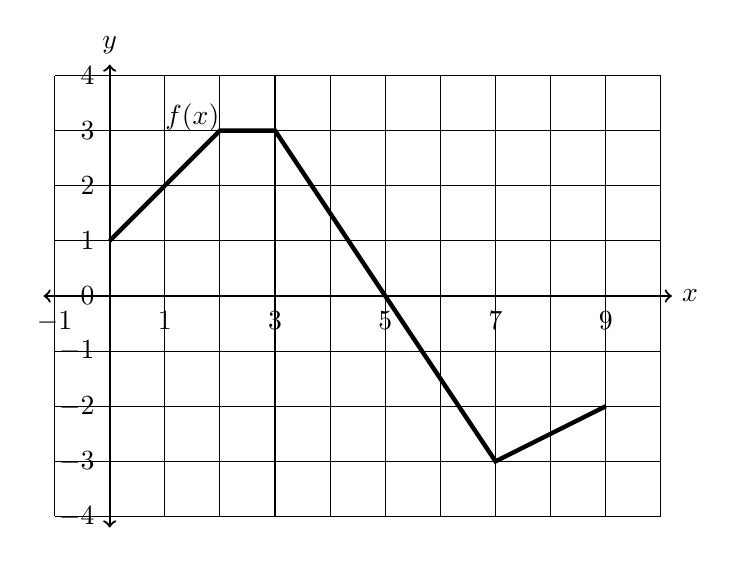
\begin{tikzpicture}[scale = .7]
\draw[<->,  thick](-1.2,0) -- (10.2,0) node[right]{$x$};
\foreach \i in {-1,1, ..., 10}{\draw (\i,.1) -- (\i, -.1) node[below]{$\i$};}
\draw[<->,  thick](0,-4.2) -- (0,4.2) node[above] {$y$};
\foreach \i in {-4, ..., 4}{\draw (.1, \i) -- ( -.1,\i) node[left]{$\i$};}
\draw[thin] (-1,-4) grid (10,4);
\draw[ultra thick] (0,1) -- (2,3) -- (3,3) -- (7,-3)--(9,-2);
\draw (1.5,2.8) node[above] {$f(x)$};
\end{tikzpicture}
\end{adjustbox}




%\vfill
\item  Using the fact that $\d \int_0^1 x^2 dx = \frac 1 3$ and $\d \int_{1}^{2} x^{2}\ dx = \frac{7}{3}$,
evaluate the following using the properties of integrals. 

  \begin{multicols}{3}{
      % make sure you added \usepackage{enumerate}
      \vspace*{-0.45in}
      \begin{enumerate}[(a)]
      \item $\d \int_0^1 5x^2\  dx$
      \item $\d \int_0^1 ( 4 + 3x^2)\ dx$
       \item $\d \int_0^2 x^{2}\ dx$. 
      \end{enumerate}}
  \end{multicols}
\vfill
\end{enumerate}
\end{document}
